\section{Access Modifiers}

\begin{frame}[fragile]{Access modifiers}
\pause
\begin{minted}[fontsize=\footnotesize]{python}
student = Student("Daan", "Wichmann", "secret", "secret")
\end{minted}
\pause
\begin{minted}[fontsize=\footnotesize]{python}
print(student.s_number)
>>> "secret"
student.s_number = "different"
print(student.s_number)
>>> "different"
\end{minted}
\end{frame}

\begin{frame}{Access modifiers: the problem}
\begin{itemize}
    \item However, s-numbers generally shouldn't change!
    \item And if they do, we want to control how they change
    \item How do we fix this? \textbf{Access modifiers}
\end{itemize}
\end{frame}

\begin{frame}{Access modifiers}
    \begin{block}{Access modifiers}
        Access modifiers control the visibility (access) of the methods and data attributes of a class.
    \end{block}
\end{frame}

\begin{frame}{Access modifiers}
\begin{itemize}
    \item Access modifiers specify from where we can access our data attributes/methods, meaning:
    \begin{itemize}
        \item for \textbf{methods}: where we can call them
        \item for \textbf{data attributes}: where we can access them (get them), and where we can change them (set them)
    \end{itemize}
\end{itemize}
\end{frame}

\begin{frame}[fragile]{Access modifiers}
\begin{itemize}
    \item We can modify access to our data attributes and methods at three levels:
    \begin{itemize}
        \item public
        \item protected
        \item private
    \end{itemize}
    \item Data attributes and methods are public by default
\end{itemize}
\end{frame}

\begin{frame}{The different of access}
\begin{tabular}{rccc}
 & Inside the class & In derived classes & Outside the class\\\hline
\textbf{public} & Yes & Yes & Yes \\
\textbf{protected} & Yes & Yes & No \\
\textbf{private} & Yes & No & No \\
\end{tabular}
\pause
\begin{itemize}
    \item Remember this table!!!!
\end{itemize}
\end{frame}

\begin{frame}{How to modify access???}
We can change the access modifier of a data attribute/method by changing the name:
\begin{itemize}
    \item s\_number (public)
    \item \_s\_number (protected)
    \item \_\_s\_number (private)
\end{itemize}
\pause
We change the number of underscores before the name!
\begin{itemize}
    \item public = 0 underscores
    \item protected = 1 underscore
    \item private = 2 underscores
\end{itemize}
\end{frame}

\begin{frame}[plain]
Lets update our student class
\end{frame}

\begin{frame}[fragile]{Modifying the access}
\begin{minted}[fontsize=\footnotesize]{python}
class Student(Person):
    def __init__(self, first_name, last_name, age, s_number):
        super().__init__(first_name, last_name, age)
\end{minted}
\pause
\begin{minted}[fontsize=\footnotesize]{python}
        self.__s_number = s_number  # We added two underscores
\end{minted}
\pause
\begin{minted}[fontsize=\footnotesize]{python}

# This part is outside the class
student = Student("Daan", "Wichmann", 21, "s1234567")
print(student.__s_number)
\end{minted}
\begin{itemize}
    \item Is s\_number a public, protected or private attribute?
    \pause
    \item Can we print it here?
\end{itemize}
\end{frame}

\begin{frame}[fragile]{Modifying the access}
\begin{minted}[fontsize=\footnotesize]{python}
class Student(Person):
    def __init__(self, first_name, last_name, age, s_number):
        super().__init__(first_name, last_name, age)
        self.__s_number = s_number  # We added two underscores

    def talk(self):
        print(f"Student {self.__s_number} is talking")
\end{minted}
\begin{itemize}
    \item Can we access it here?
\end{itemize}
\end{frame}

\begin{frame}{Remember our hierarchy}
    \begin{figure}
        \centering
        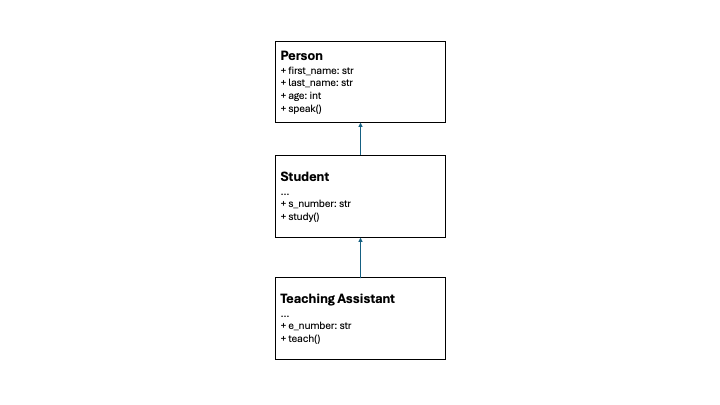
\includegraphics[scale=0.30]{images/hierarchy.png}
        \caption{our hierarchy}
        \label{fig:focuslogo}
    \end{figure}
\end{frame}

\begin{frame}[fragile]{Modifying the access}
\begin{minted}[fontsize=\footnotesize, breaklines]{python}
class Student(Person):
    def __init__(self, first_name, last_name, age, s_number):
        super().__init__(first_name, last_name, age)
        self.__s_number = s_number

# TeachingAssistant derives from Student
class TeachingAssistant(Student)
    def __init__(self, first_name, last_name, age, s_number, e_number):
            # Calling the constructor of Student
            super().__init__(first_name, last_name, age, s_number)
            self.__e_number = e_number

    def talk(self):
        print(f"Student {self.__s_number} is talking")
\end{minted}
\begin{itemize}
    \item Can we access it here?
\end{itemize}
\end{frame}

\begin{frame}[fragile]{Modifying the access again}
\begin{minted}[fontsize=\footnotesize, breaklines]{python}
class Student(Person):
    def __init__(self, first_name, last_name, age, s_number):
        super().__init__(first_name, last_name, age)
        self._s_number = s_number  # Removed one underscore

class TeachingAssistant(Student)
    def __init__(self, first_name, last_name, age, s_number, e_number):
            # Calling the constructor of Student
            super().__init__(first_name, last_name, age, s_number)
            self.__e_number = e_number

    def talk(self):
        print(f"Student {self._s_number} is talking")
\end{minted}
\begin{itemize}
    \item Is s\_number public, private or protected?
    \pause
    \item Can we access it in TeachingAssistant now?
\end{itemize}
\end{frame}

\begin{frame}[fragile]{Back to being private}
\begin{minted}[fontsize=\footnotesize, breaklines]{python}
class Student(Person):
    def __init__(self, first_name, last_name, age, s_number):
        super().__init__(first_name, last_name, age)
        self.__s_number = s_number  # It's private again!

class TeachingAssistant(Student)
    def __init__(self, first_name, last_name, age, s_number, e_number):
            # Calling the constructor of Student
            super().__init__(first_name, last_name, age, s_number)
            self.__e_number = e_number

    def change_student_number(self, new_student_number):
        self.__s_number = new_student_number
\end{minted}
\begin{itemize}
    \item Can we do this?
    \pause
    \item Not being able to access it, means we also shouldn't change it!
\end{itemize}
\end{frame}

\begin{frame}{Python being Python}
    \pause
    \begin{alertblock}{Access modifiers in Python (only for technical details)}
        In Python, access modifiers are not heavily enforced. Meaning, that if we wanted to, we can still access private/protected data attributes in places we shouldn't. However, it is the convention that you shouldn't! (And in the exam it is assumed they are heavily enforced).
    \end{alertblock}
    \begin{itemize}
        \item Other languages like Java, do heavily enforce their access modifiers.
    \end{itemize}
\end{frame}

\begin{frame}{Why are we doing this again?}
\begin{itemize}
    \item Why are we making our data attributes and methods private or protected?
    \pause
    \item \textbf{Encapsulation}
\end{itemize}
\end{frame}